\section{The Mess We Are In}

\begin{quotex}
The idea that nature is a closed system of natural causes and that natural causes provide a complete account of everything that occurs in nature is deeply entrenched in the West. \flright{\textsc{William Dembski}}

\end{quotex}
The common sentimental idea is that the Garden of Eden was set up perfectly for Adam. This cannot be the case as it stands. The natural world existed as such, which we still experience. Adam was given supernatural graces that could never be given to animals, plants, and minerals. But animals still lived natural lives, and there were natural dangers from fire, and other events.

Moreover, Adam had preternatural abilities. Although preternatural abilities are beyond nature, Adam was the agent (not God). These abilities intrude willy-nilly into life even in our time, so we can presume Adam had more control over them. They go by the names paranormal, psychic, second sight, and so on. If they exist, their occurrences seem to be mostly random.

Adam's natural abilities were enhanced. So he was always aware of what was going on and was never distracted. His ability to think logically and act rationally were unimpaired. The reason I express it this way is to show that if the primordial state cannot be an aspiration, at least it can be understood (at least to the initiated).

There is no point to turn Adam into some sort of Prometheus as though we can now ``think for ourselves". If that is so, the results have been completely underwhelming.

\paragraph{Fallen State}
The soul is spiritual and corporal. The former transcends the world and the latter is tied to the body and its function. The Fall indicates that the center of being descends from the Self of the spirit soul to the Ego of the corporal soul. The Self is forgotten and largely subconscious, or better said, superconscious. The attributes of the Primordial State are suddenly transformed:

\begin{itemize}
\item \textbf{Knowledge} $\Rightarrow $ Ignorance, stupidity, opinion (in place of gnosis) 
\item \textbf{Integrity} $\Rightarrow $ inner confusion, lying to self and others, deception, doubt 
\item \textbf{Impassibility} $\Rightarrow $ motivated by unhealthy emotions and disordered desires. Malice and Concupiscence 
\item \textbf{Immortality} $\Rightarrow $ Death, with associated fear and anxiety 
\end{itemize}
The Fall is never total, and there is always the possibility of access to the higher attributes.

\paragraph{Fallen World}
Multiply that by 7.6 thousand million and we have the modern world. Ignorance, malice, and concupiscence used to be considered faults to be overcome, like this

\begin{itemize}
\item Education to overcome ignorance 
\item Control of emotions to overcome malice 
\item Moderation to overcome excessive desire. 
\end{itemize}
That is no longer the case. Propaganda replaces education. Malice is encouraged as a method of social control. Hardly any sexual desire is considered anti-social and even gluttony is defended.

\begin{wrapfigure}{rt}{.3\textwidth}
 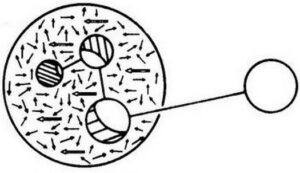
\includegraphics[scale=.5]{a20200909TheMessWeAreIn-img001.jpg}
 \caption{World influences}
 \end{wrapfigure}

The world, then, is ruled by conflicting opinions, not to mention outright falsehoods. This situation is represented in the diagram by small arrows going in random directions. These are called the ``A" influences. If you remember your vector math, you can see that the sum of all the vectors amounts to zero. That means that the entire world process, under these A influences, is going nowhere.

That is the global view. However, locally there may be clusters of A influences that are aligned together. In that section of the world, they can wield power because any opposition, being disorganized, again sums up to zero. Eventually, even that apparent unity dissipates into its opposite.

There are always attempts within the world process that promise unity. Thus, science, philosophy, political programs are proposed, but never achieve the goal. Science, for example, is simply too difficult for the majority of people to understand, and its conclusions—never really definitive—are perverted for political purposes.

The idea that there will be a scientific, philosophical, or political solution to the problems of human life—some day in the distant future—is widespread among the educated class. It is considered a marker for intelligence, despite all available historical evidence. For the person who comes to terms with this, there are two choices

\begin{enumerate}
\item Nihilism, the notion that there is no ultimate truth 
\item The solution must arise from outside the world process system 
\end{enumerate}
So that is the ultimate result of Adam's hubris to determine good and evil for himself. He can remain delusional, admit that his project ended in failure, or seek to return to the Primordial State that he had rejected.

\paragraph{Nausea and Repetition}
I sent the little ones youtube videos of one-celled animals eating each other, disintegrating, cloning themselves. The kids were delighted, especially the ones with microscopes. But I wondered why. For perhaps hundreds of millions of years, these critters have been reproducing the same drama over and over and over again. Eating, dying, attacking, reproducing for no purpose. Nauseating.

The ducks wandering about the neighbourhood are the same. Occasionally, one will nest and lay eggs behind the bushes around my house. A dozen ducklings hatch. They leave the nest, all following the mother. The next day some are missing. More missing on the day after. Maybe one or two reach adulthood just to start the cycle over again.

Who can live like that? But human life is no different. The same little dramas repeat and repeat, just with minor variations on the theme. A confessor used to ask me about Moses' neighbour. Who dat I asked. Exactly. No one cares about Moses' neighbour anymore. Ever since then, the same stories, the same situations, the same sins. Just different people, all 50 billion of them soon forgotten. Multi-celled paramecia.

\paragraph{The Way Out}
In the diagram, notice the longer and larger arrows all pointing in the same direction from right to left. These represent the influences of revealed religion. Some people, in despair, will respond to those B influences; the remainder will continue their neverending battles of opinion. Those exoteric influences show the path to escape the world process. For a few, there are the C or esoteric influences. Although the B influences are sufficient in themselves, the C (and higher) influences can lead to even higher states of being.

\paragraph{Infallible}
Obviously, to be of any benefit, these higher influences are necessarily infallible. The way out of the mess cannot be just one more opinion among the others. It will be countercultural, much different from the way the world thinks and acts.

Many are offended at the notion of infallibility. I can't understand why. I haven't met many people who would concede that their opinions about all manner of things might possibly be incorrect.

Many others will become interested in this Revelation. So they will read books about it, seek out teachers, even idolize their favourite authors. They will know much about the way out, and how predecessors described the way out, but they seldom bother to actually tread the path.

A few will claim to guide you on the way out, but they are wolves in sheep's clothing. They will often tell you how wonderful you are. And all the time how wonderful they are.

\paragraph{Salvation}
The story is misunderstood if it only about living in a perfect environment, like a mouse utopia. That is insufficient, because even the serpent inhabits the garden. Evil, therefore, was a possibility of manifestation, so it manifested. Salvation is something else, something much greater than the garden. And it involves the serpent, but that is another story.



\flrightit{Posted on 2020-09-09 by Cologero }

\begin{center}* * *\end{center}

\begin{footnotesize}\begin{sffamily}



\texttt{Thomas on 2020-09-09 at 12:33 said: }

``Adam's natural abilities were enhanced. So he was always aware of what was going on and was never distracted. His ability to think logically and act rationally were unimpaired."

How did he ``fall" then ?


\hfill

\texttt{Cologero on 2020-09-09 at 16:49 said: }

You need to read it to the end, and also in conjunction with the previous post.

I don't mind the conversation, though, because maybe some points can be clarified.


\hfill

\texttt{Sylvan Savant on 2020-09-11 at 16:25 said: }

This might sound irrelevant but please bear with me. Everyone has likely heard of the MGTOW movement. Basically these are jaded men who came to the shocking realization that women are essentially insufferable. 

Man has a certain idea in his mind about what a woman is, and when that idea doesn't correspond with empirical reality, he begins to make a generalization about what their genuine nature must be like. Some of them might even go to the extremes of delving into the age old perceptions of witches and skin changers, which I won't go into here. Besides, the reality of woman as a object that is sensed may be one thing, but how they are perceived by two different people is an entirely different matter.

This is especially true of a highly attractive woman, who since childhood, quickly finds out that certain things are ``expected" of her from male company. This prevents her from putting forth a sincere impression of what she actually is in front of people, which further complicates matters.

In any case this isn't about women, but about perception. Already you can see here how brittle is the notion we live in a empirical reality the nature of which is entirely rationally intelligible. 

Zhuge Liang was a very lucky man. His wife was hard working, loyal, intensely loving and they both had a shared taste for poetry. She was also incredibly plain. Not ugly, or even uncomely, just plain. I wonder how many times Zhuge had to fight back a feeling of insufferable regret as he turned down the advances of the many gorgeous women of the Shu court?

We can't say beauty is just skin deep. Actually in my opinion this is untenable even if it is true. To repeat the age old adage of ``value integrity over appearance" may be wise, but it is practically speaking useless. This is because beauty is a window into the world beyond. Beauty makes no sense from a utilitarian point of view, it has no explanation from a naturalist perspective and it is inimic by nature to randomness and chance.

Of course a scientist would say that beauty is nothing but an evolutionary adaptation to a vital external stimulus, such as hunger or mating on one hand, and on the other hand a neurochemical-behavioral response that the need to satisfy such things prompt. This is akin to giving attributes to the higher functions of the mind in terms of the brain stem. The problem with that explanation is that science talks about what is perceived, but this isn't the reality that man finds himself in, nor can it ever be. Rather he inescapably finds himself trapped in the internal world of unperceived images, unrealized passions and unfulfillable desires. 

To continuously grasp after them is his lot in life, in the only way that he knows how, through the acquisition of the fleeting experience that their facsimiles and reproductions can provide in the sensible world. Hence you have the modern world defining life as this verminous chase after money, women, cars, video game achievements, radical political ideologies and so on. We are all like this without exception. Breaking out of this state is unbelievably easy, but it requires a radical change in understanding of our nature, which is why it is impossible for most people. 

This brings us back to the fall. In the end, you can't escape from the truth as laid out in the Scriptures, no matter how diligently one might try ridicule and trample it.


\hfill

\texttt{Cologero on 2020-09-13 at 14:35 said: }

Good thoughts, Sylvan, but we are discussing quite different things. I am not as interested in the empirical, but rather in the psychological and even metaphysical. We may have many images of women in our heads, especially in our time when we are bombarded by images. Keep in mind that historically images were hard to come by.

The task of the alchemical marriage (from the male point of view) is to identify the true Anima and to distinguish it from all the false ideas. That, it turns out, is not so easy. Most men will reject the notion entirely, and it is not at all about ``getting in touch with the feminine side".

As for Zhuge Liang: I don't want to be too explicit but a man has within himself a very reliable and objective judge of who is physically attractive enough. In any case, a man's life project cannot revolve around a woman. If he found a loving companion who would make the circumstances of his life more comfortable, then he was quite fortunate. He was considered intelligent and wise, so perhaps he is a good example to follow.


\hfill

\texttt{Thomas on 2020-09-14 at 10:02 said: }

You said that " Evil, therefore, was a possibility of manifestation, so it manifested." The question is why was it a " possibility of manifestation ‘ rather than ( to use the same terminology ) a possibility of non-manifestation ?


\hfill

\texttt{Cologero on 2020-09-14 at 10:38 said: }

Tom, that is a very good question and the answer may be more complex than it seems. … assuming there is a good answer.

The serpent was in the supposedly perfect garden for some reason, so the possibility of a dual mind or doubt was baked into creation.

So why was evil manifested? There is the notion that evil is somehow not ultimately ``real", and that it is merely the absence of good. That seems to imply that evil as such cannot be manifested.

Even if that is the case from the metaphysical point of view, it is not satisfying from the psychological point of view. Jung points that out and analyzes various symbols on that topic. The effects of evil certainly feel real.

Augustine wanted to avoid the Manichaeism that he left behind. It raised evil up to the level of the good, so there is an ongoing cosmic battle between god and evil. On the other side, movements like Christian Science or ACIM take the notion to the extreme and deny the reality of sickness, evil, etc.

I'm gathering material on the topic will post it when ready.

In the meantime, interiorly we can experience that same dual mind.


\hfill


\end{sffamily}\end{footnotesize}
